%! Author = adnansiddiquei
%! Date = 28/06/2024

\section{Model Training}\label{sec:training}
\begin{figure}[t]
    \centering
    \makebox[\textwidth]{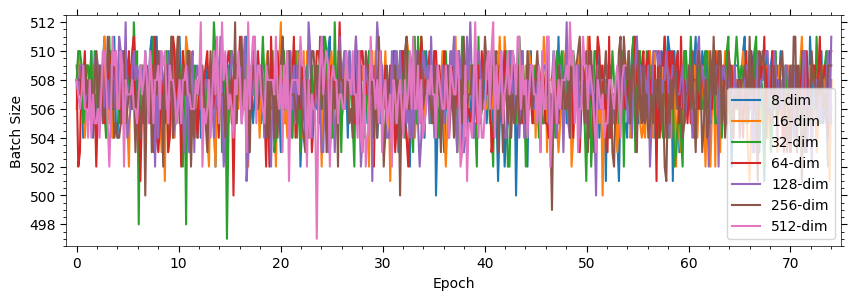
\includegraphics[width=0.9\textwidth]{figures/train_batch_size}}
    \caption{The batch size for each batch after the pre-processing steps were applied to the batch on the fly.
    Each line represents the batch size throughout the training of AstroCLIP models with everything identical except the
    embedding dimensionality.
    The individual lines are not meant to be discernable from one another, but rather this figure should show the general trend.}
    \label{fig:train_batch_size}
\end{figure}

\begin{figure}[t]
\centering
\begin{subfigure}{1\textwidth}
  \centering
  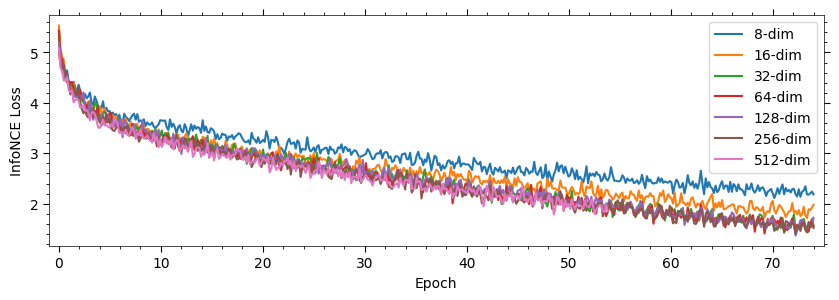
\includegraphics[width=0.9\linewidth]{figures/train_loss}
  \caption{Training loss.}
  \label{fig:train_loss}
\end{subfigure}%
\hfill
\begin{subfigure}{1\textwidth}
  \centering
  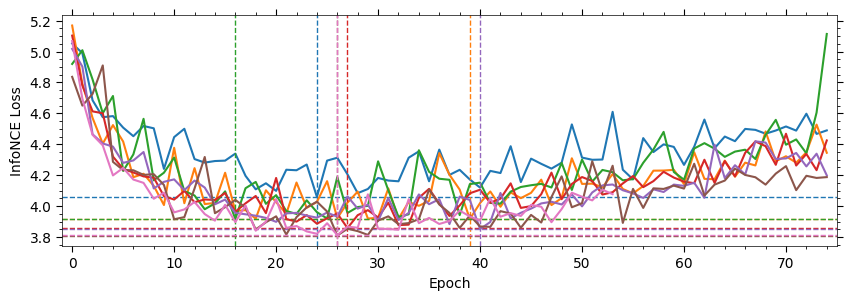
\includegraphics[width=0.9\linewidth]{figures/val_loss}
  \caption{Validation loss.
  The vertical lines correspond to the epoch at which the lowest validation loss was achieved and the horizontal
  line corresponds to the loss value at that epoch.
  The (embedding dimensionality, lowest validation loss, epoch) values are as follows: (8, 4.06, 24); (16, 3.92, 39);
  (32, 3.92, 16); (64, 3.86, 27); (128, 3.85, 40); (256, 3.81, 26); (512, 3.81, 26).}
  \label{fig:val_loss}
\end{subfigure}
\caption{Train and validation loss for AstroCLIP models with varying embedding dimensionality.
The legend on Figure~\eqref{fig:train_loss} applies to both plots.}
\label{fig:train_val_loss}
\end{figure}

Our AstroCLIP model unifies these two embedders into a single model, and then fine-tunes the embeddings using the InfoNCE loss
(Equation~\eqref{eq:infonce}).
The embedding dimensionality was varied through the range $[8, 16, 32, 64, 128, 256, 512]$ and each model was trained for
75 epochs.
Through some exploratory analysis, we fixed a few hyperparameters: batch size of 512; learning rate of $5e^{-4}$; a weight
decay of $1e^{-4}$; and a temperature parameter in the InfoNCE loss of 0.07; and only varied the embedding dimensionality.
One small aspect of note is that the batch size was not consistent throughout training, the pre-processing mentioned in
Section~\eqref{subsec:pre-processing} was performed on the fly on each batch of data as and when randomly sampled by
the DataLoader during training.
This meant that there were small fluctuations in the batch size, and for completeness we show the batch size for each batch
throughout the training of the AstroCLIP models in Figure~\eqref{fig:train_batch_size}.
As can be seen on the figure, the batch size fluctuates very little and generally remains between 502 and 510.
This fluctuating batch size was intentionally left in the training process as it's effects were negligible and would likely
only have a positive effect through the stochasticity it introduces.
The number of epochs required to reach the lowest validation loss, and the corresponding loss is detailed in Figure~\eqref{fig:val_loss}.
Whilst there is a clear pattern in the training loss where the more flexible model appears to be able to achieve the
lowest loss, the same was not true for the validation loss with no clear pattern emerging.
However, it is important to note that a thorough sweep of hyperparameters was not performed, and so it is possible that
a different set of hyperparameters (such as stronger regularisation on the more flexible models, to prevent over-fitting)
could have yielded different results (lower validation loss for the more flexible models).
